\documentclass[a3paper]{article}
\usepackage[left=0mm,top=1cm,right=0mm,bottom=0mm]{geometry}
% \documentclass[border=0]{standalone}
\usepackage{tikz}
\usepackage{xcolor}
\definecolor{pGreen}{HTML}{006633}
\definecolor{sgbGreen1}{HTML}{66cc99}
\definecolor{sgbGreen2}{HTML}{ccffcc}

\definecolor{pRed}{HTML}{cc0033}
\definecolor{sgbRed}{HTML}{cc6688}
\definecolor{sgbRed2}{HTML}{FF99CC}

\definecolor{sgbGrey}{HTML}{333333}
\definecolor{sgbGrey2}{HTML}{996666}
\definecolor{sgbGrey3}{HTML}{999966}

\begin{document}
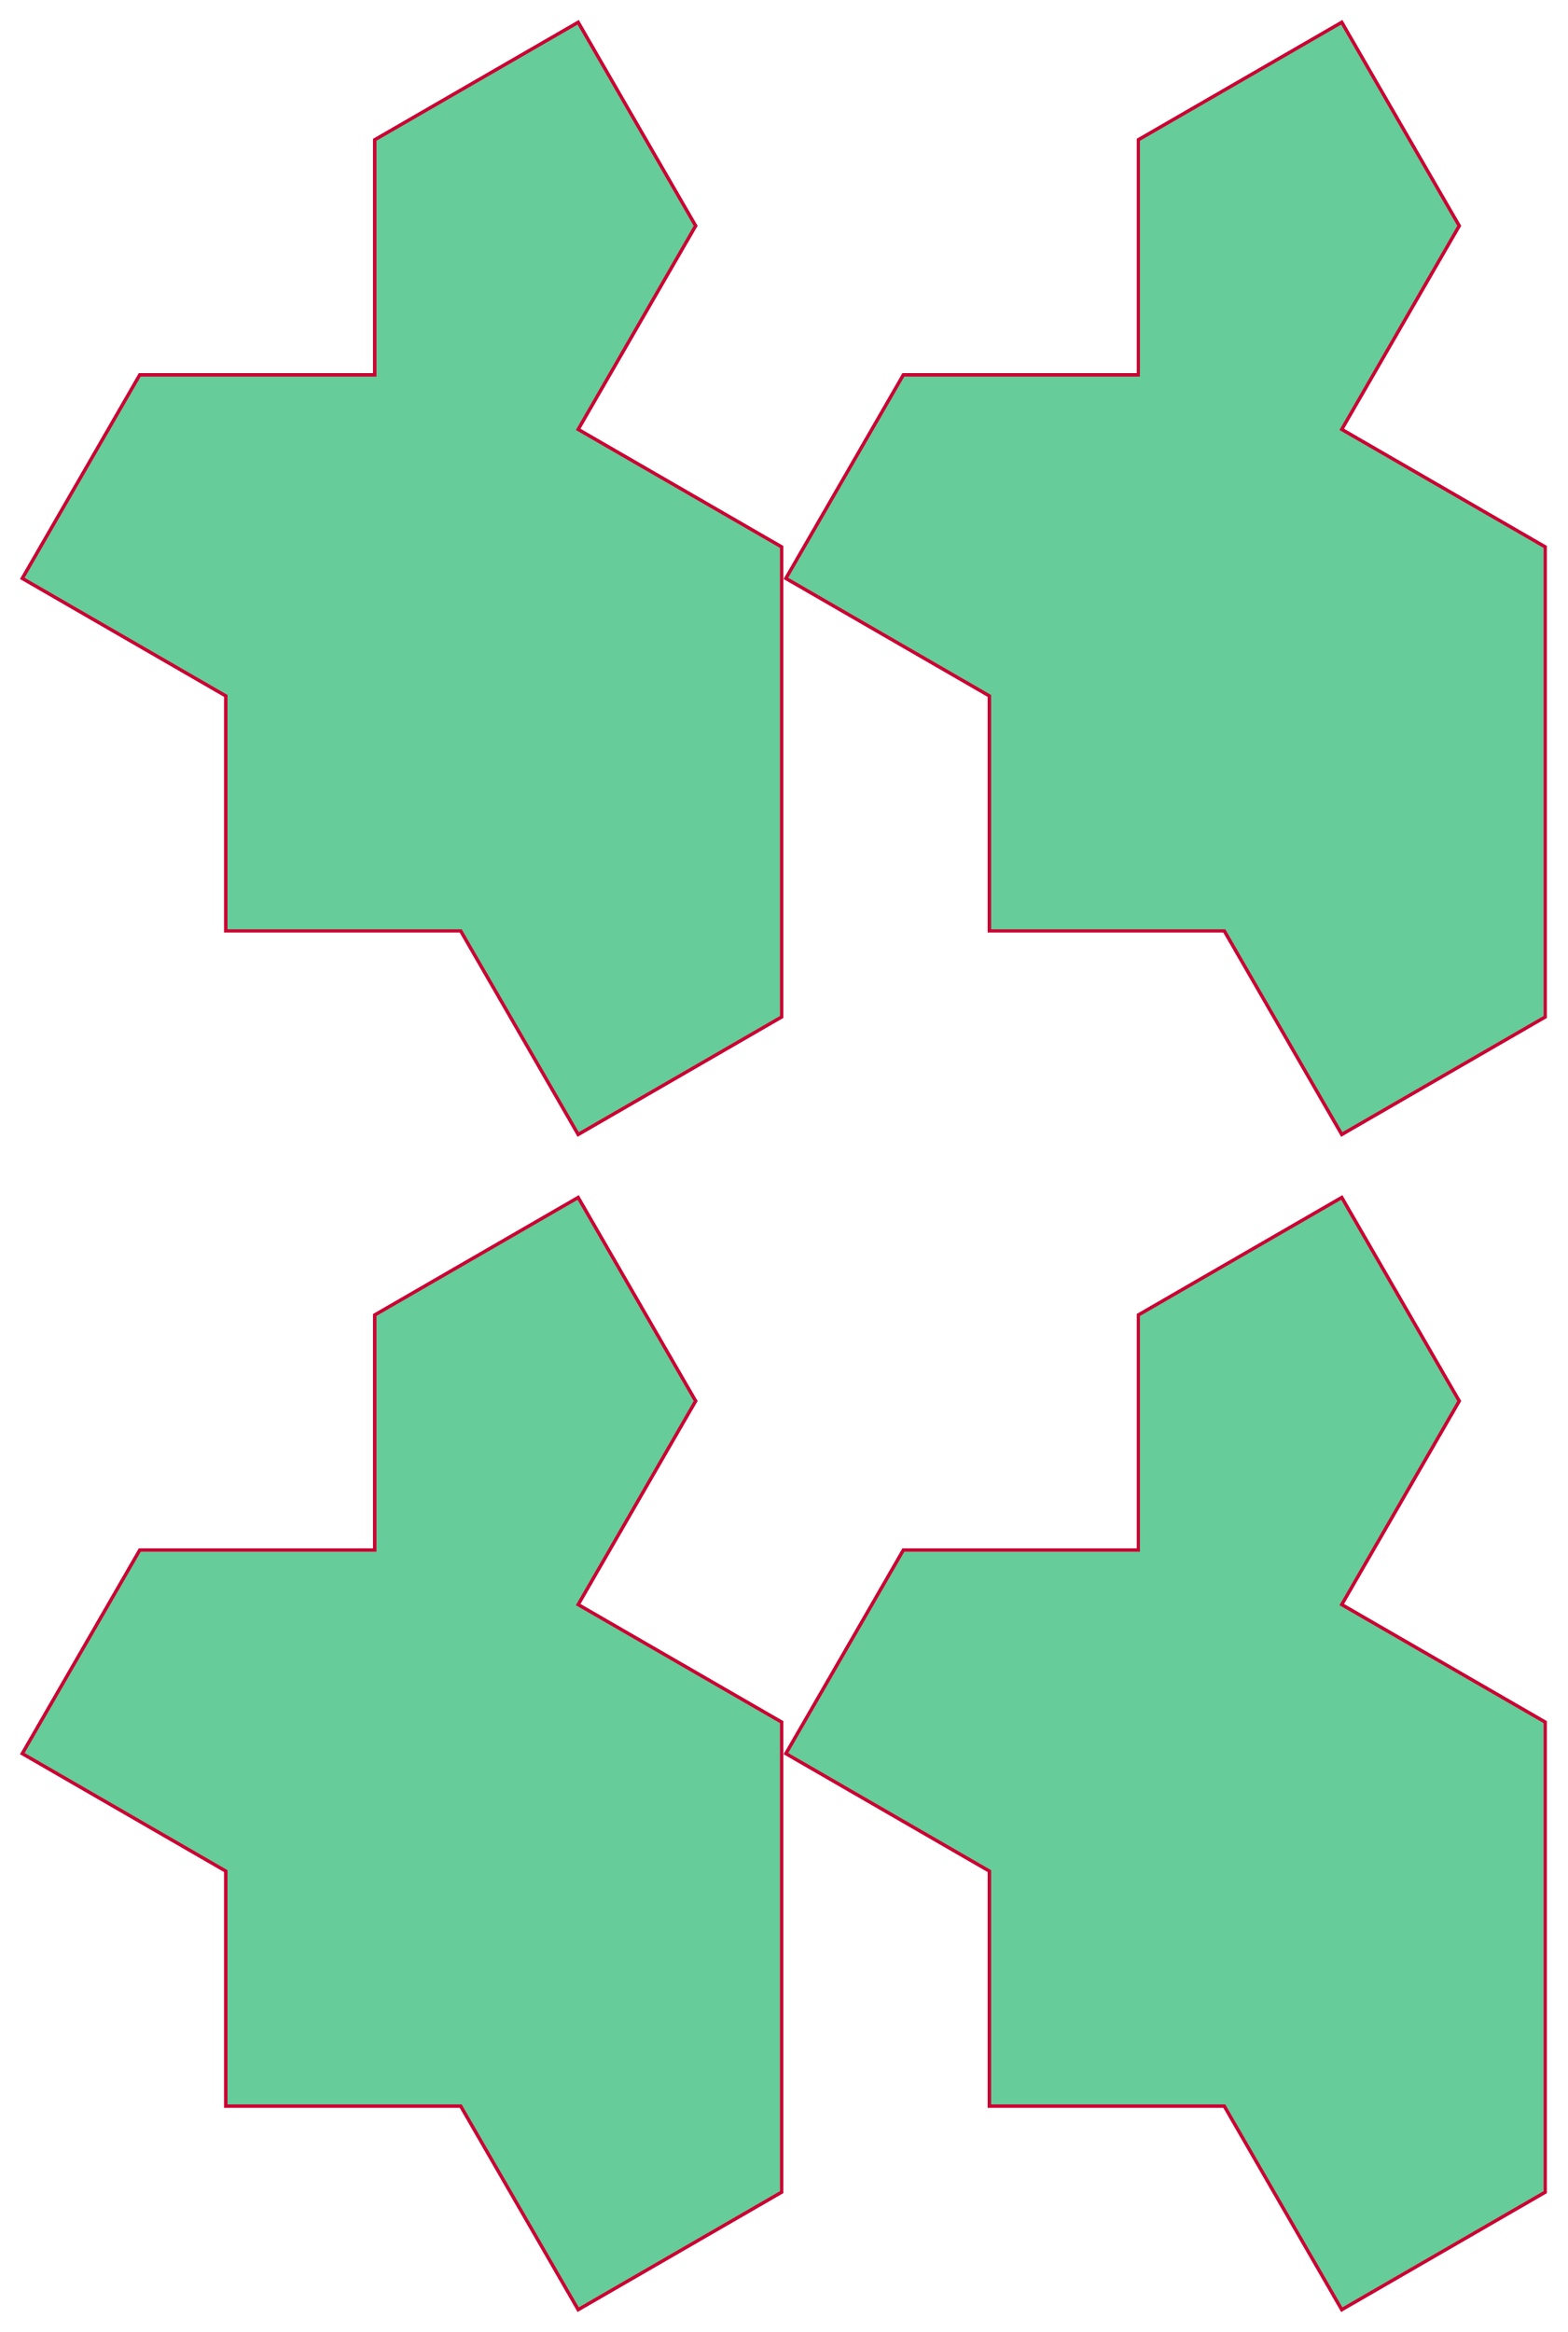
\begin{tikzpicture}
    \pgfmathsetmacro{\w}{4}
    \tikzset{
        tile11/.pic={
            \filldraw[sgbGreen1,draw=pRed,ultra thick] (0,0) --++(-90:\w)--++(0:\w)--++(-60:\w)--++(30:\w)--++(90:{2*\w})--++(150:\w)--++(60:\w)--++(120:\w)--++(-150:\w)--++(-90:\w)--++(180:\w)--++(-120:\w)--cycle;
        }
    };
    \draw(0,0) pic {tile11};
    \draw(0,20) pic {tile11};
    \draw(13,0) pic {tile11};
    \draw(13,20) pic {tile11};
\end{tikzpicture}
\end{document}